% IDEIA INICIAL:
%   Ideia inicial dos métodos;
%   Propriedades
%   Exemplos de métodos:
%       Euler Simplético (1a Ordem);
%       Velocity-Verlet (2a Ordem);
%       Ruth3 e Ruth4 (3a e 4a Ordem);
%       RKN551 e RKN671 (5a e 6a Ordem);
%       SVCP8S15 e SVCP10S35 (8a e 10a Ordem).
%   Comparacao numerica com os métodos tradicionais;

\section{Integradores simpléticos}\label{secao:integradores_simpleticos}
Como apresentado brevemente na introdução deste capítulo, os métodos simpléticos se baseiam na estrutura do espaço de fases, e não apenas na função que está sendo integrada. Nesse sentido, tais métodos são construídos de modo a preservarem a estrutura simplética dos problemas hamiltonianos, conservando o volume da solução e consequentemente conservando as integrais primeiras também.

Essas diferenças na forma e objetivo de construir os integradores entre os métodos tradicionais e os simpléticos têm implicações importantes sobre os resultados. Os métodos tradicionais são construídos tendo-se em vista uma estabilidade assintótica do sistema, imbuindo dissipações na solução numérica que distorcem as trajetórias de sistemas hamiltonianos, ainda que sejam aplicados integradores tradicionais de alta ordem, como exemplificado ao final da seção anterior. Isso não ocorre com integradores simpléticos, como apresentamos a seguir.

Para esta seção, no lugar de considerar um problema de Cauchy qualquer, tomaremos aqueles que podem ser escritos através das equações de Hamilton:
\begin{equation}\label{eq:pvi_hamilton}
    \dvet z(t) = \bm \Omega \nabla_{\vet z} H(\vet z),
    \quad
    \vet z(0) = \vet z_0,
    \quad
    \vet z(t) = (\vet q(t), \vet p(t)),
    \quad
    \bm \Omega = \begin{bmatrix}
        \bm 0 & \bm I \\ - \bm I & \bm 0
    \end{bmatrix}.
\end{equation}

Como já apresentado no capítulo \ref{capitulo:revisao_mecanica}, o fluxo do problema (\ref{eq:pvi_hamilton}) é \textit{simplético}, ou seja, conserva o volume no espaço de fases. Em particular, isso significa que conserva também as integrais primeiras do sistema. A proposta dos \textit{integradores simpléticos} é fornecer uma aplicação simplética $\vet \Phi_h$ tal que
\begin{equation*}
    \vet z_1 = \vet \Phi_h(\vet z_0).
\end{equation*}
Ademais, conforme o teorema \ref{teorema:simpleticidade_matricial}, um critério para $\vet \Phi_h$ ser simplética é ser tal que
\begin{equation*}
    D \Phi_h \bm \Omega D \Phi_h^T = \bm \Omega.
\end{equation*}


\subsection{Obtenção de métodos via separação}
Quando a função hamiltoniana é separável, ou seja, $H(\vet q, \vet p) = T(\vet p) + V(\vet q)$, é possível obter métodos explícitos a partir do que segue. Tomando como hamiltoniano primeiramente apenas $T$ e em seguida apenas $V$, temos os dois problemas de valor inicial respectivos:
\begin{equation}
    \begin{cases}
        \dvet q = \nabla_{\vet p} T(\vet p) = \dfrac{1}{m} \vet p, \\
        \dvet p = \vet 0,
    \end{cases},
    \quad
    \begin{cases}
        \dvet q = \vet 0, \\
        \dvet p = - \nabla_{\vet q} V(\vet q) = F(\vet q).
    \end{cases}   
\end{equation}
Em ambos os casos, podemos obter o fluxo de maneira explícita, uma vez que uma das coordenadas está constante:
\begin{equation}
    \vet \Phi_{\tau, T} (\vet z) = \begin{bmatrix}
        \vet q + \tau \vet p/m \\ \vet p
    \end{bmatrix},
    \quad
    \vet \Phi_{\tau, V} (\vet z) = \begin{bmatrix}
        \vet q \\ \vet p + \tau \vet F(\vet q)
    \end{bmatrix}.
\end{equation}
Se tomamos a aplicação composta $\vet \Phi_{\tau} := \vet \Phi_{\tau, T} \circ \vet \Phi_{\tau, V}$, obtemos um primeiro método com semblante familiar.

\begin{method}[Euler Simplético (ou semi-implícito)]\label{metodo:euler_simpletico}
    Para um tamanho de passo $h$ fixo em um intervalo discretizado para um problema de valor inicial hamiltoniano separável, temos a aproximação:
    \begin{equation}
        \vet q_{k+1} = \vet q_k + h \dfrac{\vet p_{k+1}}{m},
        \quad
        \vet p_{k+1} = \vet p_k + h \vet F(\vet q_k).
    \end{equation}
\end{method}

Da mesma forma que os métodos de Euler explícito e implícito (métodos \ref{metodo:euler_explicito} e \ref{metodo:euler_implicito}, respectivamente), o método de Euler simplético tem ordem 1 \citep[189]{Hairer2006-oz}. No entanto, trata-se de um método simplético, pois vale o critério matricial (Teorema \ref{teorema:simpleticidade_matricial}):
\begin{equation*}
    D \vet \Phi_h = \begin{bmatrix}
        1 + \dfrac{h^2}{m} \nabla_{\vet q} \vet F(\vet q) & \dfrac{h}{m} \\
        h \nabla_{\vet q} \vet F(\vet q) & 1
    \end{bmatrix}
    \quad
    \Longrightarrow
    \quad
    D \vet \Phi_h \bm \Omega D \vet \Phi_h^T = \begin{bmatrix}
        \vet 0 & \bm I \\ - \bm I & \vet 0
    \end{bmatrix}
    = \bm \Omega.
\end{equation*}

A diferença entre os métodos pode ser observada aplicando-os no problema-modelo \ref{probmodelo:lemniscata}, como na figura \ref{fig:var_energia_rk22_rk33_rk44_es}. Veja que embora todos os métodos de Runge-Kutta (com ordem maior que 1) comecem com uma variação menor de energia que o método de Euler simplético (com ordem 1), a variação do segundo é relativamente preservada, enquanto que a dos métodos RK escalona. No caso do RK44, embora a precisão seja mantida por mais tempo para $h=0.05$, um tamanho de passo $h=0.15$ permite visualizar melhor o erro na energia escalonando.

\begin{figure}
    \centering
    \begin{subfigure}{.5\textwidth}
      \centering
      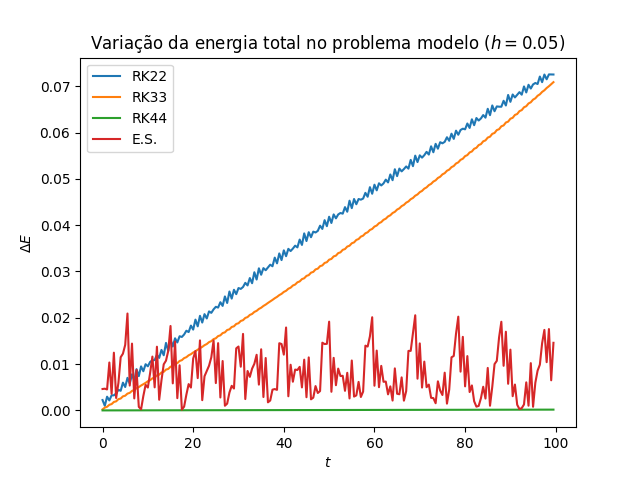
\includegraphics[width=\linewidth]{tcc/img/var_energia_rk22_rk33_rk44_es.png}
      \caption{Intervalo $[0,100]$ e $h=0.05$.}
      \label{fig:var_energia_rk22_rk33_rk44_es_a}
    \end{subfigure}%
    \begin{subfigure}{.5\textwidth}
      \centering
      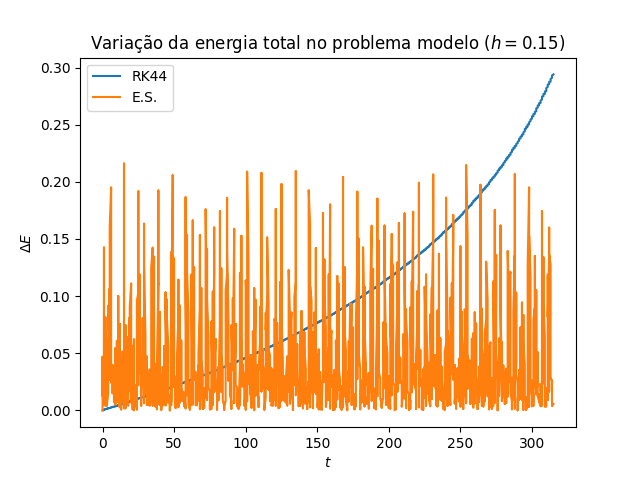
\includegraphics[width=\linewidth]{tcc/img/var_energia_rk44_es.png}
      \caption{Intervalo $[0,300]$ e $h=0.15$.}
      \label{fig:var_energia_rk22_rk33_rk44_es_b}
    \end{subfigure}
    \caption{Variação da energia total na simulação do problema-modelo \ref{probmodelo:lemniscata} com os métodos RK22, RK33, RK44 e Euler Simplético (E.S.)}
    \label{fig:var_energia_rk22_rk33_rk44_es}
\end{figure}

A ideia de composição também pode ser aplicada para obter métodos com ordem mais alta. Tomando constantes de peso (isto é, que somam 1) $c_1, ..., c_s$ e $d_1, ..., d_s$, tomamos a composição
\begin{equation*}
    \vet \Phi_h = \vet \Phi_{d_s h, V} \circ \vet \Phi_{c_s h, T} \circ \hdots \circ \vet \Phi_{d_1 h, V} \circ \vet \Phi_{c_1 h, T}.
\end{equation*}
Conforme \cite[145-146]{Leimkuhler2005}, métodos $\vet \Phi_h$ com esta forma são consistentes e, além disso, se os coeficientes são simétricos ($c_i = c_{s+1-i}$ e $d_i = d_{s+1-i}$), então o método tem no mínimo ordem 2.

\begin{method}[Velocity-Verlet]\label{metodo:velocity-verlet}
    Tomando os coeficientes $d_1=d_2=1/2$, $c_1 = 0$ e $c_2=1$, obtemos um método consistente, simétrico, explícito, simplético e de segunda ordem dado por
    \begin{align*}
        \vet q_{k+1} &= \vet q_k + h \dfrac{\vet p_k}{m} + \dfrac{h^2}{2 m} \vet F(\vet q_k), 
        \\
        \vet p_{k+1} &= \vet p_k + \dfrac{h}{2} (\vet F(\vet q) + \vet F(\vet q_{k+1})).
    \end{align*}
\end{method}

\begin{theorem}
    O método Velocity-Verlet é simplético.
\end{theorem}
\begin{Proof}
    Seja $\vet \Phi_h (\vet q, \vet p) = (\vet Q (\vet q, \vet p), \vet P(\vet q, \vet p))$. Então:
    \begin{align*}
        \derpar{\vet Q}{\vet q} &= 1 + \dfrac{1}{2} \dfrac{h^2}{m} \derpar{\vet F}{\vet q}, 
        &\quad
        \derpar{\vet Q}{\vet p} &= \dfrac{h}{m}, 
        \\
        \derpar{\vet P}{\vet q} &= \dfrac{h}{2} \derpar{\vet F}{\vet q} \left(1 + \derpar{\vet Q}{\vet q}\right),
        &\quad
        \derpar{\vet P}{\vet p} &= \derpar{\vet Q}{\vet q}.
    \end{align*}
    Nesse caso, a condição do teorema \ref{teorema:simpleticidade_matricial} é facilmente verificada:
    \begin{equation*}
        \derpar{\vet Q}{\vet q} \derpar{\vet P}{\vet p} - \derpar{\vet Q}{\vet p} \derpar{\vet P}{\vet q} 
        = \left(\derpar{\vet Q}{\vet q}\right)^2 - \left(\derpar{\vet Q}{\vet q} - 1\right) \left(1 + \derpar{\vet Q}{\vet q}\right) = 1.
    \end{equation*}
\end{Proof}

Outros dois métodos de ordens 3 e 4 foram propostos, respectivamente, por \cite{Ruth1983} e por \cite{Forest1990}.

\begin{method}[Ruth 3]\label{metodo:ruth3}
    Um método simplético de 3ª ordem é obtido através dos coeficientes
    \begin{align*}
        c_1 = 1,    & \quad & c_2 = -2/3, & \quad & c_3 = 2/3, \\
        d_1 = -1/24 & \quad & d_2 = 3/4,  & \quad & d_3 = 7/24.
    \end{align*}
\end{method}

\begin{method}[Ruth 4]\label{metodo:ruth4}
    Um método simplético de 4ª ordem é obtido através dos coeficientes
    \begin{align*}
        c_1 = c_4 = \dfrac{1}{2(2-2^{1/3})}, & \quad & c_2 = c_3 = \dfrac{1-2^{1/3}}{2(2-2^{1/3})}, \\
        d_1 = d_3 = \dfrac{1}{2-2^{1/3}}, & \quad & d_2 = - \dfrac{2^{1/3}}{2-2^{1/3}}, \quad d_4 = 0.
    \end{align*}
\end{method}


\subsection{Métodos via composição de integradores de segunda ordem}
Seguindo nessa linha, \cite{Yoshida1990} observa que uma forma eficiente de obter métodos de alta ordem para problemas com funções hamiltonianas separáveis é através da composição de métodos simétricos de segunda ordem. A facilidade vem dos termos ímpares da expansão de Taylor se anularem, o que simplifica as condições de ordem do método, e procurar por métodos de ordem par é conveniente uma vez que os métodos simétricos sempre têm ordem par e são reversíveis no tempo \citep[147]{Leimkuhler2005}. Vale ressaltar que a composição de simplectomorfismos é também simplectomorfa, o que significa que compôr métodos de Verlet, por exemplo, com uma boa escolha de pesos, fornece integradores simpléticos, simétricos, consistentes e de alta ordem. Nesse caso, as aplicações compostas $\vet \Psi_h$ têm a forma
\begin{equation*}
    \vet \Psi_h = \vet \Phi_{\gamma_s h} \circ \hdots \circ \vet \Phi_{\gamma_2 h} \circ \Phi_{\gamma_1 h},
\end{equation*}
onde $\vet \Phi_{\gamma_i h}$ é o método de Verlet (\ref{metodo:velocity-verlet}) com tamanho de passo $\gamma_i h$, para $i=1,2,...,s$. Dois métodos deste tipo foram implementados no programa final, com ordens 8 e 10.

\begin{method}[svcp8s15]\label{metodo:svcp8s15}\citep[157]{Hairer2006-oz}
    Um método Stormer-Verlet Composto de 8ª ordem e 15 estágios (svc8s15) é obtido através dos coeficientes:
    \begin{center}
        \begin{tabular}{ccccr}        
        $\gamma_1$ &$=$& $\gamma_{15}$ &$=$& $0.74167036435061295344822780$ \\
        $\gamma_2$ &$=$& $\gamma_{14}$ &$=$& $-0.40910082580003159399730010$ \\
        $\gamma_3$ &$=$& $\gamma_{13}$ &$=$& $0.19075471029623837995387626$ \\
        $\gamma_4$ &$=$& $\gamma_{12}$ &$=$& $-0.57386247111608226665638773$ \\
        $\gamma_5$ &$=$& $\gamma_{11}$ &$=$& $0.29906418130365592384446354$ \\
        $\gamma_6$ &$=$& $\gamma_{10}$ &$=$& $0.33462491824529818378495798$ \\
        $\gamma_7$ &$=$& $\gamma_{9}$  &$=$& $0.31529309239676659663205666$ \\
                   &   & $\gamma_{8}$  &$=$& $-0.79688793935291635401978884$ \\
        \end{tabular}
    \end{center}
\end{method}

\begin{method}[svcp10s35]\label{metodo:svcp10s35}\citep[158]{Hairer2006-oz}
    Um método Stormer-Verlet Composto de 10ª ordem e 35 estágios (svc8s15) é obtido através dos coeficientes:
    \begin{center}
        \begin{tabular}{ccccr}        
        $\gamma_1$  &$=$& $\gamma_{35}$ &$=$& $ 0.07879572252168641926390768$ \\
        $\gamma_2$  &$=$& $\gamma_{34}$ &$=$& $ 0.31309610341510852776481247$ \\
        $\gamma_3$  &$=$& $\gamma_{33}$ &$=$& $ 0.02791838323507806610952027$ \\
        $\gamma_4$  &$=$& $\gamma_{32}$ &$=$& $-0.22959284159390709415121340$ \\
        $\gamma_5$  &$=$& $\gamma_{31}$ &$=$& $ 0.13096206107716486317465686$ \\
        $\gamma_6$  &$=$& $\gamma_{30}$ &$=$& $-0.26973340565451071434460973$ \\
        $\gamma_7$  &$=$& $\gamma_{29}$ &$=$& $ 0.07497334315589143566613711$ \\
        $\gamma_8$  &$=$& $\gamma_{28}$ &$=$& $ 0.11199342399981020488957508$ \\
        $\gamma_9$  &$=$& $\gamma_{27}$ &$=$& $ 0.36613344954622675119314812$ \\
        $\gamma_{10}$ &$=$& $\gamma_{26}$ &$=$& $-0.39910563013603589787862981$ \\
        $\gamma_{11}$ &$=$& $\gamma_{25}$ &$=$& $ 0.10308739852747107731580277$ \\
        $\gamma_{12}$ &$=$& $\gamma_{24}$ &$=$& $ 0.41143087395589023782070412$ \\
        $\gamma_{13}$ &$=$& $\gamma_{23}$ &$=$& $-0.00486636058313526176219566$ \\
        $\gamma_{14}$ &$=$& $\gamma_{22}$ &$=$& $-0.39203335370863990644808194$ \\
        $\gamma_{15}$ &$=$& $\gamma_{21}$ &$=$& $ 0.05194250296244964703718290$ \\
        $\gamma_{16}$ &$=$& $\gamma_{20}$ &$=$& $ 0.05066509075992449633587434$ \\
        $\gamma_{17}$ &$=$& $\gamma_{19}$ &$=$& $ 0.04967437063972987905456880$ \\
                    &   & $\gamma_{18}$ &$=$& $ 0.04931773575959453791768001$ \\
        \end{tabular}
    \end{center}
\end{method}

Apesar da relativa facilidade de obter métodos simpléticos através de composição de métodos de primeira e de segunda ordem, é fácil ver pelos métodos \ref{metodo:svcp8s15} e \ref{metodo:svcp10s35} que é necessária uma quantidade de estágios muito maior do que a ordem do método, o que torna a usabilidade dos métodos cada vez mais desafiadora. Porém, existem muitos outros métodos simpléticos e que não são baseados em composição. Dois tipos bastante comuns são os métodos de Runge-Kutta Simpléticos e os métodos de Runge-Kutta-Nyström.

\subsection{Métodos de Runge-Kutta Simpléticos e de Runge-Kutta-Nyström}
Para obter um método de Runge-Kutta simplético basta adicionar uma restrição (além das já apresentadas anteriormente) sobre o método \ref{metodo:rk_r_estagios}.

\begin{theorem}\label{teorema:rk_simpletico}
    Se os coeficientes de um método de Runge-Kutta de $R$ estágios são tais que
    \begin{equation*}
        b_i a_{ij} + b_j a_{ji} - b_i b_j = 0, \quad i, j = 1, ..., R, 
    \end{equation*}
    então trata-se de um método simplético.
\end{theorem}

A demonstração do teorema pode ser encontrada em \cite[152-154]{Leimkuhler2005}. O importante neste momento é que decorre do teorema que para $i=j$ temos
\begin{equation*}
    2 a_{ii} = b_i, \quad \forall i = 1, 2, ..., R.
\end{equation*}
Uma vez que o vetor $\vet b$ não é nulo, isso significa que a matriz de coeficientes $\bm A$ tem diagonal não-nula, e portanto não é possível obter um integrador de Runge-Kutta simplético que seja explícito. Tendo em vista as já mencionadas dificuldades de se trabalhar computacionalmente com métodos implícitos, nenhum método de Runge-Kutta simplético foi testado neste trabalho.

Já os métodos de Runge-Kutta-Nyström (RKN) são voltados especificamente para problemas de valor inicial do tipo
\begin{equation*}
    \ddvet x = g(t, \vet x, \dvet x),
\end{equation*}
então são aplicáveis para grande parte dos problemas de mecânica hamiltoniana, como o PNCG. O método geral é dado pelo que segue.

\begin{method}[Runge-Kutta-Nyström de $s$ estágios]\citep[41]{Hairer2006-oz}
    Um método RKN de $s$ estágios para um sistema hamiltoniano separável em $T$ e $V$ é dado por
    \begin{align*}
        \vet y_i & = \vet q_k + c_i h \dfrac{\vet p_k}{m} + h^2 \sum_{j=1}^{s} a_{ij} \dfrac{\vet F(\vet y_i)}{m}, \quad i = 1, 2, ..., s, \\
        \vet q_{k+1} &= \vet q_k + h \dfrac{\vet p_k}{m} + h^2 \sum_{i=1}^{s} b_i \dfrac{\vet F(\vet y_i)}{m}, \\
        \vet p_{k+1} &= \vet p_k + h \sum_{i=1}^{s} B_i \vet F(\vet y_i),
    \end{align*}
    para constantes $\bm A, \vet b, \vet c$ e $B_1, ..., B_s$.
\end{method}

Da mesma forma que para os métodos de Runge-Kutta, um método RKN é explícito se $a_{ij} = 0$ para $j \geq i$. Porém, existem critérios para que um método RKN explícito seja simplético \citep[376]{Okunbor1994}:
\begin{align}
    b_i &= B_i (1-c_i), &\quad 1 \leq i \leq s, \\
    a_{ij} &= B_j(c_i - c_j), &\quad j < i.
\end{align}
Dessa forma, foi possível testar métodos de Runge-Kutta-Nyström simpléticos e explícitos. Os escolhidos para teste constam em \cite{Okunbor1994} e são como segue. O número 1 sufixado ao nome dos métodos indica que, em referência às tabelas 1 e 2 de Okunbor e Skeel, tratam-se do método 1. O método RKN551 foi escolhido entre os 4 sem critérios, e o RKN671 foi escolhido por ter o menor resíduo entre os apresentados pelos autores.

\begin{method}[RKN551]\label{metodo:rkn551}
    Um método RKN de 5ª ordem e 5 estágios simplético e explícito é dado pelos seguintes coeficientes:
    \begin{table}[H]
        \centering
        \begin{tabular}{r|r}
            \multicolumn{1}{c}{$B_i$} & \multicolumn{1}{c}{$c_i$} \\
            \hline
            -1.67080892327314312060 &  0.69491389107017931259 \\ 
             1.22143909230997538270 &  0.63707199676998338411 \\ 
             0.08849515813253908125 & -0.02055756998211598005 \\ 
             0.95997088013770159876 &  0.79586189634575355001 \\ 
             0.40090379269297793385 &  0.30116624272377778837 \\
             \hline
        \end{tabular}
    \end{table}
\end{method}

\begin{method}[RKN671]\label{metodo:rkn671}
    Um método RKN de 6ª ordem e 7 estágios simplético e explícito é dado pelos seguintes coeficientes:
    \begin{table}[H]
        \centering
        \begin{tabular}{lr}
            \hline
            $B_4$           &  0.26987577187133640373 \\ 
            $B_5 = B_3$     &  0.92161977504885189358 \\ 
            $B_6 = B_2$     &  0.13118241020105280626 \\ 
            $B_7 = B_1$     & -0.68774007118557290171 \\ 
            $c_4$           &  0.50000000000000000000 \\ 
            $c_5 = 1 - c_3$ &  0.06520862987680341024 \\ 
            $c_6 = 1 - c_2$ &  0.65373769483744778901 \\ 
            $c_7 = 1 - c_1$ &  0.05586607811787376572 \\ 
            \hline
        \end{tabular}
    \end{table}
\end{method}

\subsection{Comparações entre os métodos apresentados}
A mesma ideia de verificação de ordem para os métodos tradicionais pode ser aplicada para os métodos simpléticos, como é apresentado na tabela \ref{tab:convergencia_metodos_simpleticos}. Os integradores com ordem maior que 6 geram resultados muito parecidos mesmo para os valores de $h$ relativamente grandes utilizados na tabela e mesmo quando se utiliza precisão de 128 \textit{bits}, então não pudemos verificar sua precisão com este método.

\begin{table}[]
    \centering
    \begin{tabular}{c|ccccccc}
        $h$     & E. S. & Verlet & Ruth3 & Ruth4 & RKN551 & RKN671  \\
        \hline
        $1/10$  & $1.129548$ & $1.904978$ & $3.567326$ & $3.398327$ & $5.367215$ & $5.392546$ \\
        $1/20$  & $1.057072$ & $1.974542$ & $3.659927$ & $3.840014$ & $5.869322$ & $5.836890$ \\
        $1/40$  & $1.021997$ & $1.993517$ & $3.540536$ & $3.959375$ & $5.998531$ & $5.958402$ \\
        $1/80$  & $1.008801$ & $1.998372$ & $3.361093$ & $3.989805$ & $5.948801$ & $5.989673$ \\
        $1/160$ & $1.003795$ & $1.999592$ & $3.208686$ & $3.997449$ & $5.588236$ & $6.003132$ \\
    \end{tabular}
    \caption{Convergência dos métodos no problema modelo \ref{probmodelo:lemniscata}.}
    \label{tab:convergencia_metodos_simpleticos}
\end{table}

Vale também observar a diferença na conservação da energia entre cada método simplético, pois métodos de ordem maior conservam a energia também em maior ordem. Aplicando o problema-modelo \ref{probmodelo:lemniscata} para cada método apresentado, obtemos a figura \ref{fig:var_energia_simpleticos}.

\begin{figure}
    \centering
    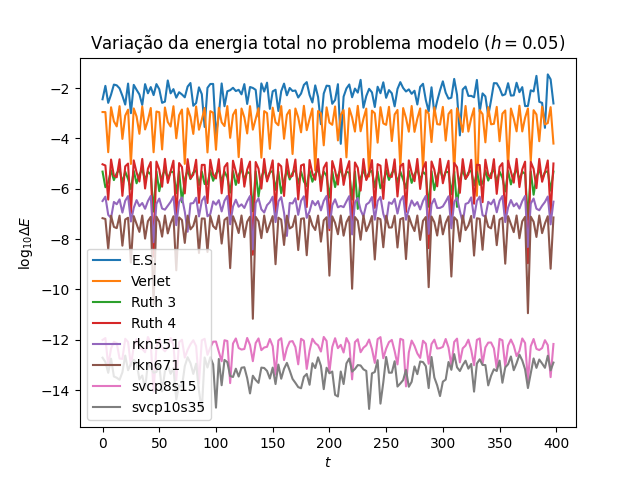
\includegraphics[width=0.7\linewidth]{tcc//img/var_energia_simpleticos.png}
    \caption{Variação da energia total para os métodos simpléticos apresentados. O problema-modelo \ref{probmodelo:lemniscata} foi integrado no intervalo $[0,400]$ com tamanho de passo $h=0.05$.}
    \label{fig:var_energia_simpleticos}
\end{figure}

Um ponto importante sobre os métodos simpléticos é que, como já dito, estes conservam não apenas a energia total, mas todas as integrais primeiras. Porém, a energia total é calculada através das velocidades e das distâncias entre os corpos, e corpos muito próximos geram instabilidade numérica no sentido de facilitarem o aparecimento de erros de ponto flutuante, enquanto as outras quantidades conservadas baseiam-se somente em operações lineares ou vetoriais diretas, sem a possibilidade de singularidades. A implicação prática disso é que as outras integrais primeiras são muito melhor conservadas que a energia total, como pode ser observado na figura \ref{fig:var_integrais_es_iau25}, na qual as outras integrais primeiras de um problema de 25 corpos possuem erro abaixo de $10^{-11}$. Dessa forma, é coerente analisar erros numéricos focando-se principalmente na energia.

\begin{figure}
    \centering
    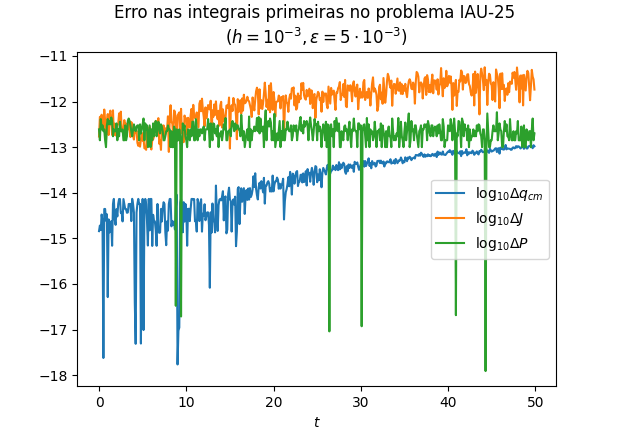
\includegraphics[width=0.5\linewidth]{tcc//img/var_integrais_es_iau25.png}
    \caption{Variação das integrais primeiras do PNCG na simulação do problema IAU-25 (\ref{probmodelo:iau25}) via método de Euler Simplético com tamanho de passo $h=10^{-3}$ e amortecimento $\epsilon=10^{-3}$. Aqui $\Delta f = |\norma{f} - \norma{f_0}|$.}
    \label{fig:var_integrais_es_iau25}
\end{figure}